\documentclass{beamer}

\usepackage[utf8]{inputenc}
\usepackage{fontspec}
\usepackage{unicode-math}

\usepackage[style=british]{csquotes}
\def\signed #1{{\leavevmode\unskip\nobreak\hfil\penalty50\hskip1em
  \hbox{}\nobreak\hfill #1%
  \parfillskip=0pt \finalhyphendemerits=0 \endgraf}}

\newsavebox\mybox
\newenvironment{aquote}[1]
  {\savebox\mybox{#1}\begin{quote}}
  {\vspace*{1mm}\signed{\usebox\mybox}\end{quote}}

\newfontfamily\DejaSans{DejaVu Sans}

\title{Glow:\\ Generative Flow with Invertible $1\times1$ Convolutions}
\subtitle{(but mainly just an introduction to normalizing flows)}
\author{Jakub Arnold}
\date{2019}

\begin{document}

\frame{\titlepage}

\begin{frame}

  \frametitle{Generative Models}

  \begin{itemize}
    \item Suppose we want to model $p(x)$, which has a complicated and
      unknown form (an image of a digit).

    \item We simplify the problem by introducing a latent variable $z$ which
      explains the context of $x$, that is $p(x | z)$ (what digit is in the image).

    \item We can still reconstruct $p(x)$ by marginalizing out $z$ while
      picking a prior $p(z)$

      \[
        p(x) = \int p(x | z) p(z)\ dz.
      \]

    \item With this in mind, we might want to ask what the latent variable
      $z$ is, given that we have an observation $x$, that is the posterior
      distribution $p(z | x)$.

    \item But unfortunately, this is intractable to compute directly, because
      it requires us to compute $p(x)$.

    % \item This is intractable, because it requires us to compute $p(x)$ which
    %   in theory could be approximated with MC integration.
    %
    %   \[
    %     p(x) \approx \frac{1}{M} \sum_{m = 1}^M p(x | z^{(m)}), z^{(m)} \sim p(z)
    %   \]
    %
    %   But this won't work in practice, because $z$ is too large.

  \end{itemize}

\end{frame}

\begin{frame}
  \frametitle{Generative Models}

  \begin{itemize}
    \item So far we've only encountered two types of generative models.
      GANs and VAEs.

    \item Neither of these learn the real data distribution $p(x)$,
      because $p(x) = \int p(x | z) p(z)\ dz$ is intractable to compute
      directly.

    \item \textbf{GAN} plays minimax and learns the distribution of data implicitly as a
      side effect.

    \item \textbf{VAE} indirectly optimizes the log-likelihood by maximizing the
      ELBO. Only learns an approximation of $p(z | x)$.

    \item \textbf{Flow-based generative models} are constructed from a sequence
      of invertible continuous transformations (with easy Jacobian determinant
      -- more on this later), and allows for exact latent variable inference.
  \end{itemize}

\end{frame}


\begin{frame}
  \frametitle{Three Types of Generative Models}

  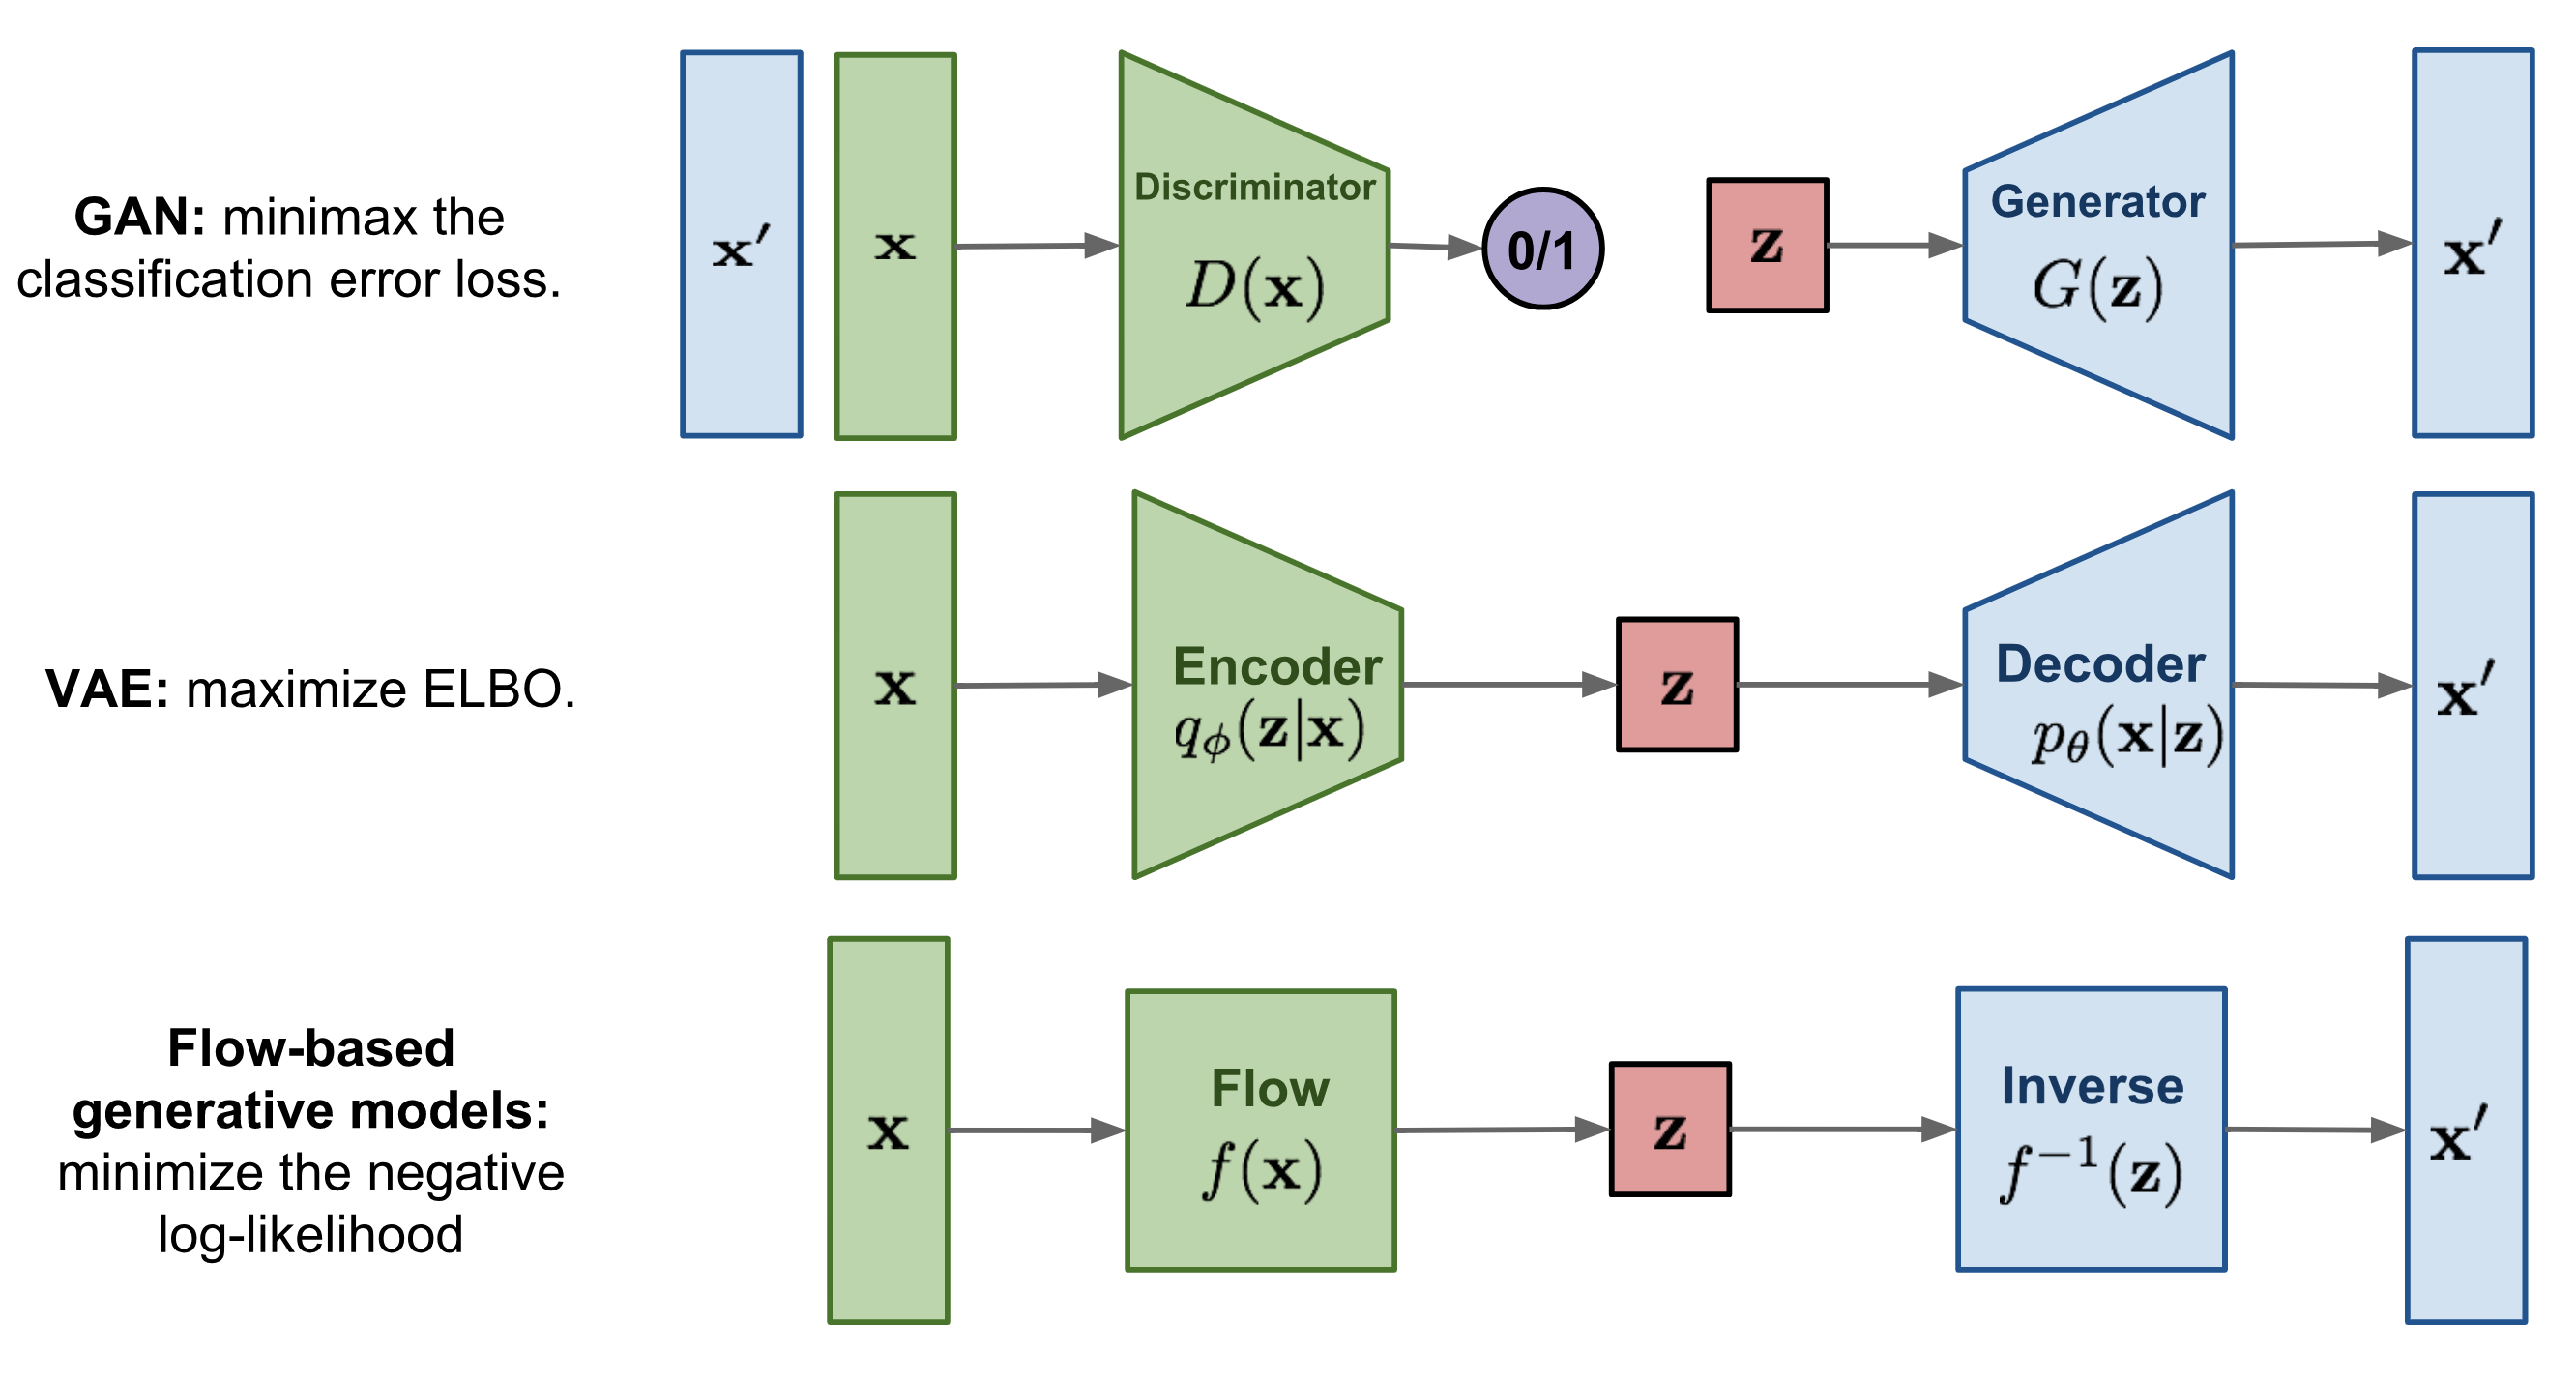
\includegraphics[width=1.0\textwidth]{three-generative-models.png}
\end{frame}

\begin{frame}
  \frametitle{Change of Variable Formula}

  Given a random variable $z$ with a known density $\pi(z)$, and an invertible
  function $x = f(z)$ (meaning we can write $z = f^{-1}(x)$).  \textbf{The question is,
  what is $p(x)$?}

  \begin{align}
    p(\textbf{x}) &= p(f(\textbf{z})) \\
                  &= \pi(f^{-1}(\textbf{x})) \cdot |\det{J(f^{-1})}|
  \end{align}

  \textbf{Proof (not really {\DejaSans 😱})}: Think of $\int \pi(z)\ dz$ as a
  sum of tiny rectangles of width $\Delta z$. Their height is the density
  $\pi(z)$. Substituting $z = f^{-1}(x)$ yields $\frac{\Delta z}{\Delta x} =
  (f^{-1}(x))'$ and $\Delta z = (f^{-1}(x))' \Delta x$, where $(f^{-1}(x))'$
  indicates the volume change between the two variables. \textbf{This extends
  to the multivariate version with the Jacobian determinant of $f$}.
\end{frame}

\begin{frame}
  \frametitle{Normalizing Flows}

  Start with a simple distribution, then apply a sequence of invertible
  transformations, applying the change of variables theorem. Because we can use
  the change of variables theorem in each step, multiplying by $|\det J(f_i)|$,
  we can recover the exact density at the end.

  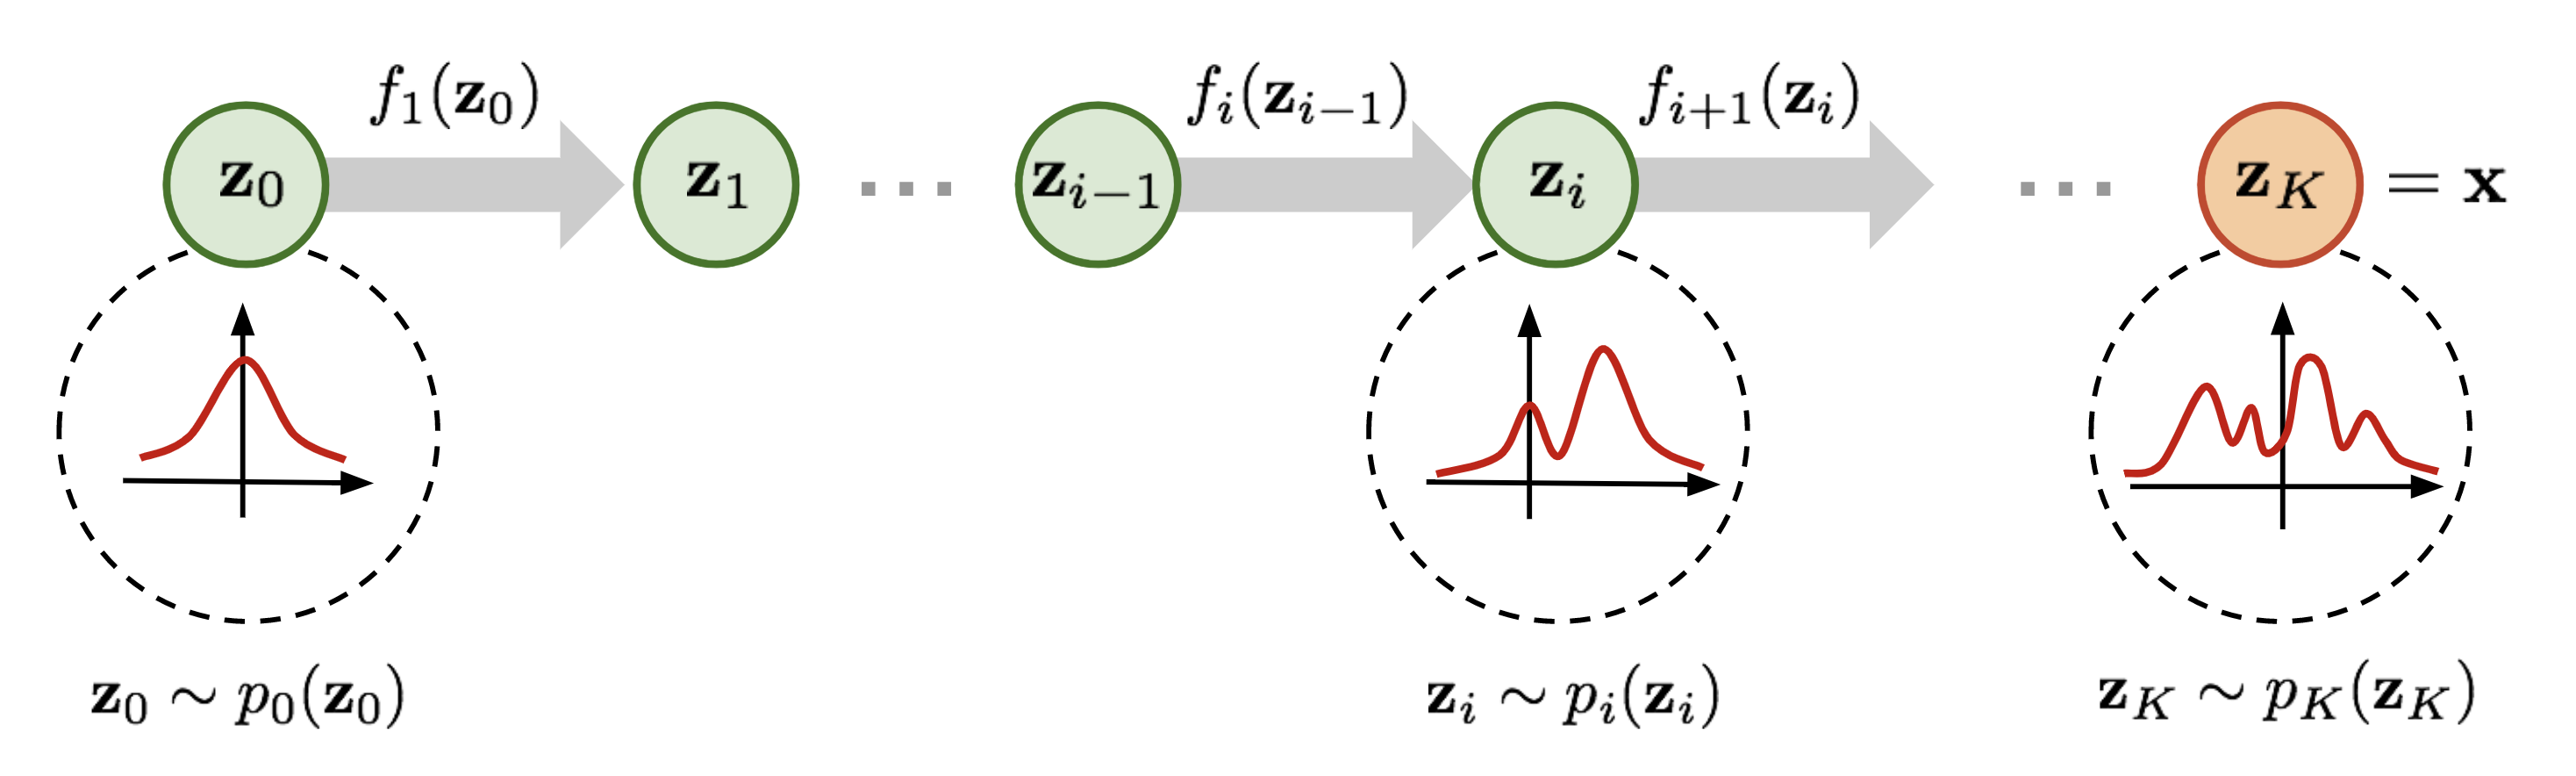
\includegraphics[width=1.0\textwidth]{normalizing-flow.png}

  The full chain is called a \textbf{normalizling flow}.
\end{frame}


\begin{frame}
  \frametitle{Normalizing Flows - Training}

  Because the exact log-likelihood $p(x)$ is tractable, we can use it to train
  the flow-based generative model by simply minimizing the negative log-likelihood
  on the training data $𝓓$:

  \[
    𝓛(𝓓) = -\frac{1}{|𝓓|} \sum_{x ∈ 𝓓} \log p(x).
  \]

  This works because we can compute $p(x)$ using the change of variables and
  because we can choose the prior $π(z)$ to be a simple tractable density, such
  as a Gaussian.

  \begin{align}
         p(x) &= π(f^{-1}(x)) |\det J(f^{-1})| \\
    \log p(x) &= \log π(f^{-1}(x)) - \sum \log |\det J(f^{-1})|
  \end{align}

\end{frame}


\begin{frame}
  \frametitle{Normalizing Flows}

  To actually compute this, we need two things:

  \begin{itemize}
    \item Easily computible inverse of $f$.
    \item Diagonal/triangular Jacobian of $f$, because $det(A)$ is $O(n^3)$.
  \end{itemize}

  If we choose $f$ such that the Jacobian is a diagonal or a triangular matrix
  $L$, we simply get $\det(L) = prod(diag(L))$.  In practice for numerical
  reasons we'll deal with log-likelihood and a log determinant.  This is even
  nicer, because $\log(\det(L)) = sum(\log(diag(L)))$.

\end{frame}


\begin{frame}
  \frametitle{Why do we care about any of this?}

  \begin{itemize}
    \item We can encode an image to $z$ and get a perfect reconstruction.

    \item In comparison, GANs don't have an encoder at all to infer $p(z | x)$.
      Unless doing something weird like VAE-GAN, which still does not optimize
      the likelihood $p(x)$.

    \item Even with a VAE, we only get an approximation of $p(z | x)$ because we're optimizing
      the lower bound on the log-likelihood. As a result, $decoder(encoder(x)) \neq x$.
  \end{itemize}
\end{frame}

\begin{frame}
  \frametitle{Glow Architecture}

  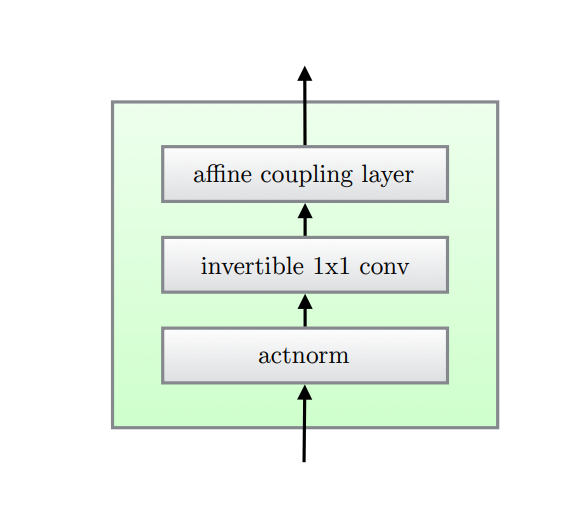
\includegraphics[width=1.0\textwidth]{glow-single-block.png}
\end{frame}

\begin{frame}
  \frametitle{Glow Layers}

  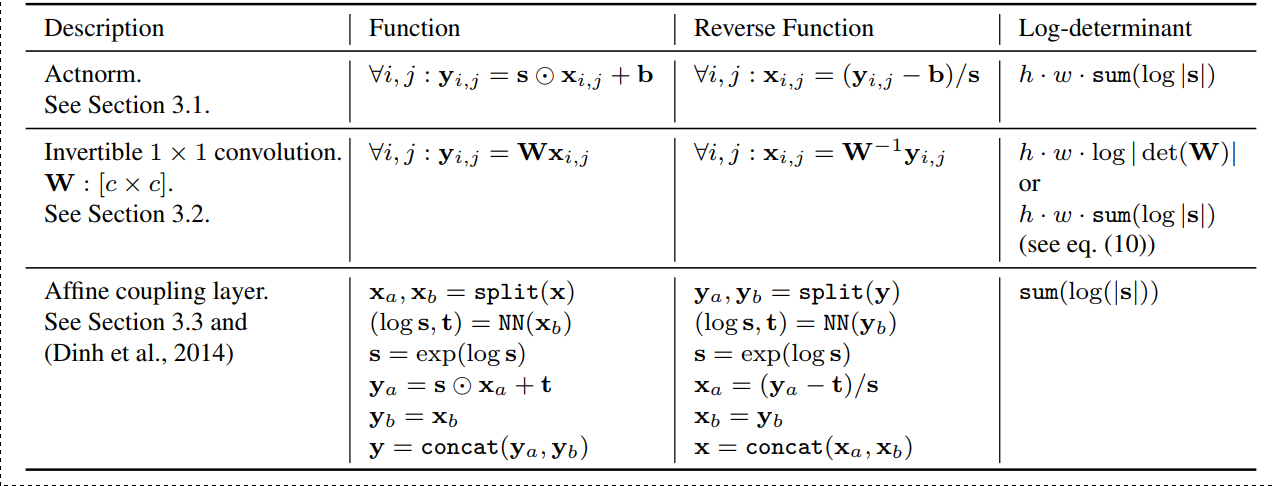
\includegraphics[width=1.0\textwidth]{glow-layers-arch.png}
\end{frame}


\begin{frame}
  \frametitle{Actnorm}

  The authors of RealNVP (previous paper, Dinh et al. 2016) suggest the use of
  batch normalization. But because Glow is too large and can only be trained
  with batch size of 1 to fit in memory, the authors of Glow propose a
  \emph{actnorm} layer (activation normalization).

  \[
    \symbf{y}_{i,j} = \symbf{s} \odot \symbf{x}_{i,j} + \symbf{b}
  \]

  \begin{itemize}
    \item Performs an affine transformation using a trainable scale and bias
      per channel.

    \item Initialized such that activations post-actnorm have zero mean and
      unit variance.

    \item After initialization, scale and bias are trained as regular trainable
      parameters.
  \end{itemize}


\end{frame}

\begin{frame}
  \frametitle{Invertible $1\times1$ convolution}

  (Dinh et al., 2014, 2016) used a fixed permutation and reversed the order of
  channels. Glow uses an invertible $1\times1$ convolution instead. This is
  done by having the same number of filters as there are input channels.

  \[
    \symbf{y}_{i,j} = \symbf{W}\symbf{x}_{i,j}
  \]

  The cost of computing $det(\symbf{W})$ is $O(c^3)$, which is comparable to the cost
  of $conv2D(\symbf{h}; \symbf{W})$, which is $O(h \cdot w \cdot c^2)$. They introduce
  a way of reducing this to $O(c)$ by using LU decomposition on $\symbf{W}$, but in the
  experiments they don't measure a significant difference in computation time.
\end{frame}

\begin{frame}
  \frametitle{Invertible $1\times1$ convolution}

  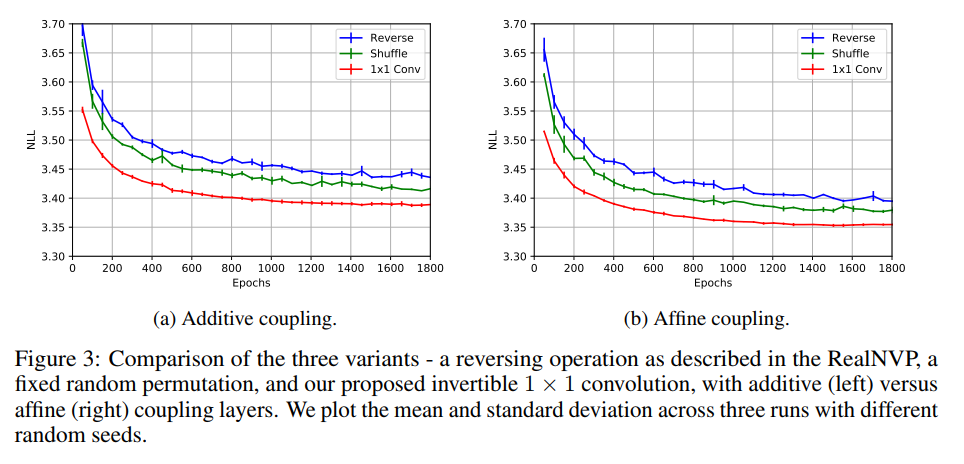
\includegraphics[width=1.0\textwidth]{conv-vs-shuffle-reverse.png}
\end{frame}

\begin{frame}
  \frametitle{Affine coupling layer}

  Since both of the previous operations are affine transformation, the affine
  coupling layer is introduced to add a non-linear (but invertible)
  transformation. Splitting $x$ into two parts along the channel dimension (in
  the code they split it in half) as $x = (x_1\  x_2)^T$ we get

  \[
    \begin{pmatrix} x_1 \\ x_2 \end{pmatrix} \rightarrow
    \begin{pmatrix} x_1 \\ s(x_1) x_2 + b(x_1) \end{pmatrix}.
  \]

  where $s$ is an invertible network. Since an activation function is an
  element-wise transformation its Jacobian is a diagonal matrix, so we just
  have to make sure it is invertible (LeakyReLU instead of ReLU, etc.).
\end{frame}

\begin{frame}
  \frametitle{Affine coupling layer}

  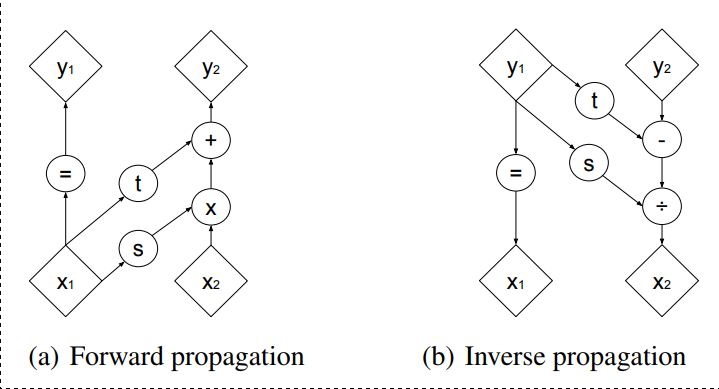
\includegraphics[width=1.0\textwidth]{glow-affine-coupling.png}
\end{frame}

\begin{frame}
  \frametitle{Affine coupling layer --- Jacobian}

  Now we just make sure we can compute the Jacobian of the affine coupling layer

  \[
    \begin{pmatrix} x_1 \\ x_2 \end{pmatrix} \rightarrow
    \begin{pmatrix} x_1 \\ x_2 s(x_1) + b(x_1) \end{pmatrix}.
  \]

  It turns out, almost as if by magic, that this is easy!

  \[
    J = \begin{pmatrix}
      \symbf{I} & 0 \\
      \frac{\partial y_2}{\partial x_1} & \frac{\partial y_2}{\partial x_2}
    \end{pmatrix} = \begin{pmatrix}
      \symbf{I} & 0 \\
      \frac{\partial y_2}{\partial x_1} & diag(s(x_1))
    \end{pmatrix}
  \]

  We don't actually have to compute $\frac{\partial y_2}{\partial x_1}$ to get $\det J$.
  Note that the $\frac{\partial y_2}{\partial x_2}$ is just $diag(s(x_1))$, because the Jacobian
  of an affine transform is a diagonal matrix.

  \href{https://github.com/kmkolasinski/deep-learning-notes/blob/master/seminars/2018-10-Normalizing-Flows-NICE-RealNVP-GLOW/notebooks/flow_layers.py}{\beamergotobutton{Affine Coupling Layer source code}}
\end{frame}

%%%%%%%%%%%%%%%%%%%%

\begin{frame}
  \frametitle{Glow Architecture}
  Each block is repeated $K$ times in a bigger block, which is repeated $L-1$
  times, wich another $K$ repeats. Set $K = 32, L = 6$.

  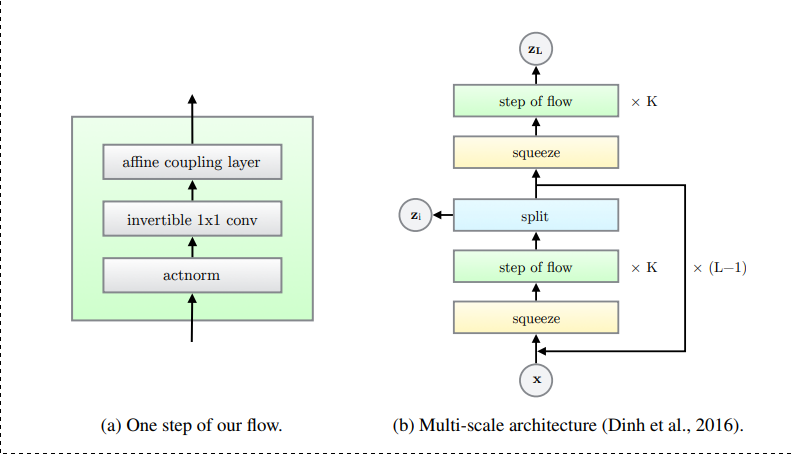
\includegraphics[width=1.0\textwidth]{glow-arch.png}
\end{frame}


\begin{frame}
  \frametitle{How big is it really?}

  \begin{itemize}
    \item Trained on 5 machines, each with 8 GPUs.
    \item \textbf{But the model is big.}
    \item They only managed to fit a minibatch of size 1 with gradient
      checkpointing (makes up to 10x bigger models fit into memory at the cost
      of increased computation).
    \item Used 5-bit images.

    \item One 256$\times$256 sample on a 1080ti takes 130ms to generate.
  \end{itemize}


\end{frame}

\begin{frame}
  \frametitle{How big is it really?}


  
\includegraphics[width=0.8\textwidth]{glow-layers.png}
\end{frame}

\begin{frame}
  \frametitle{How big is it really?}

  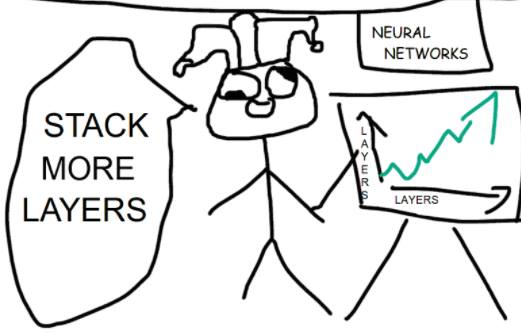
\includegraphics[width=0.8\textwidth]{layers-meme.png}
\end{frame}

\begin{frame}
  \frametitle{Glow Samples trained on CelebA HQ}

  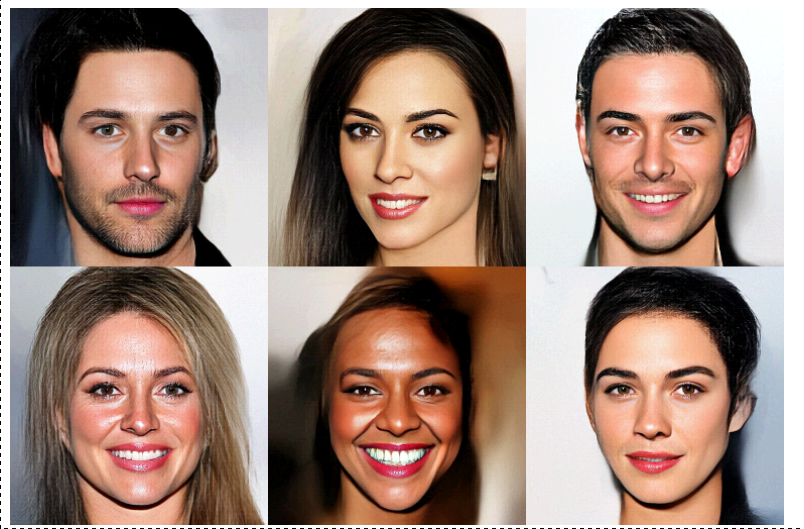
\includegraphics[width=1.0\textwidth]{glow-samples.png}
\end{frame}

\begin{frame}
  \frametitle{Glow Interpolations in $z$}

  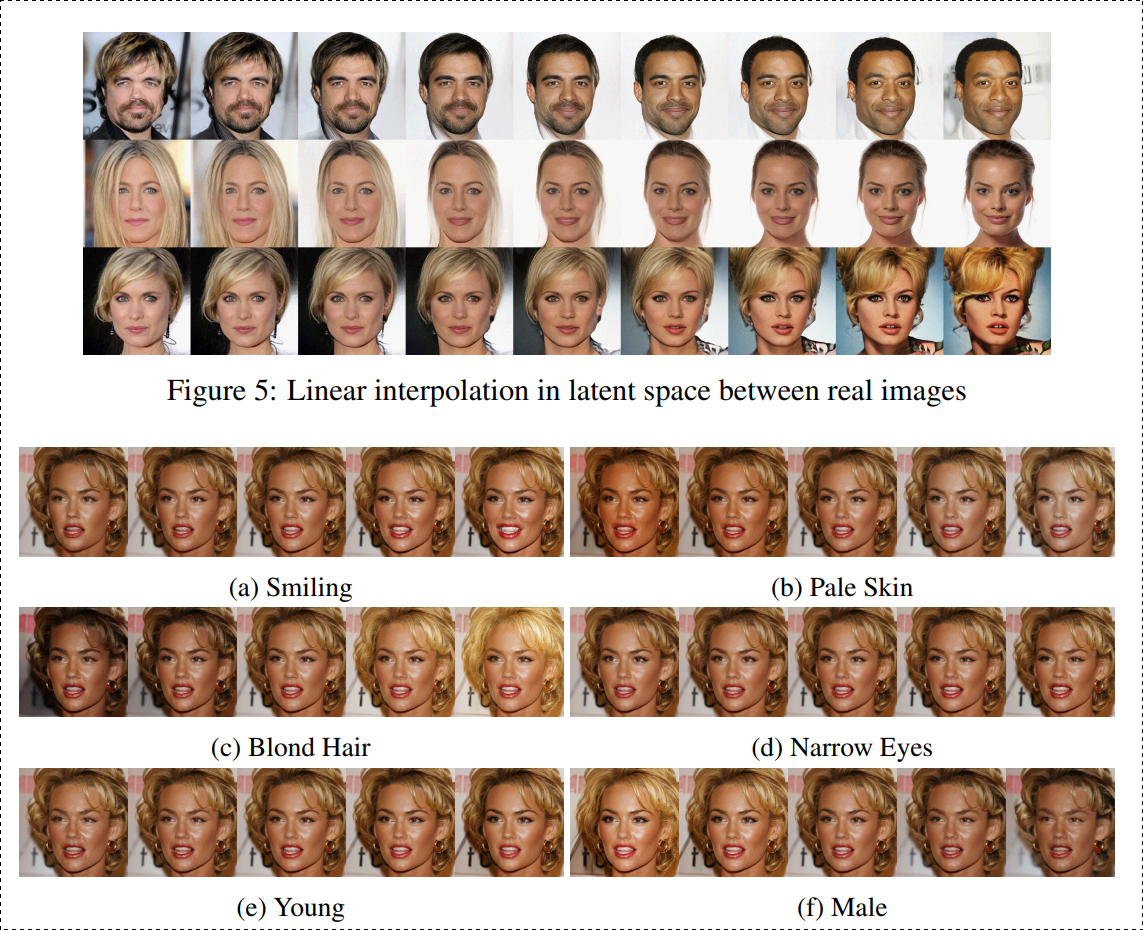
\includegraphics[width=0.9\textwidth]{glow-interpolations.png}
\end{frame}

\begin{frame}
  \begin{center}
    \Huge \href{https://openai.com/blog/glow/}{Demo}
  \end{center}
\end{frame}

\begin{frame}
  \frametitle{Effect of change in temeperature}

  Samples obtained at $0, 0.25, 0.6, 0.7, 0.8, 0.9, 1.0$ temperature. Ended up choosing $0.7$.

  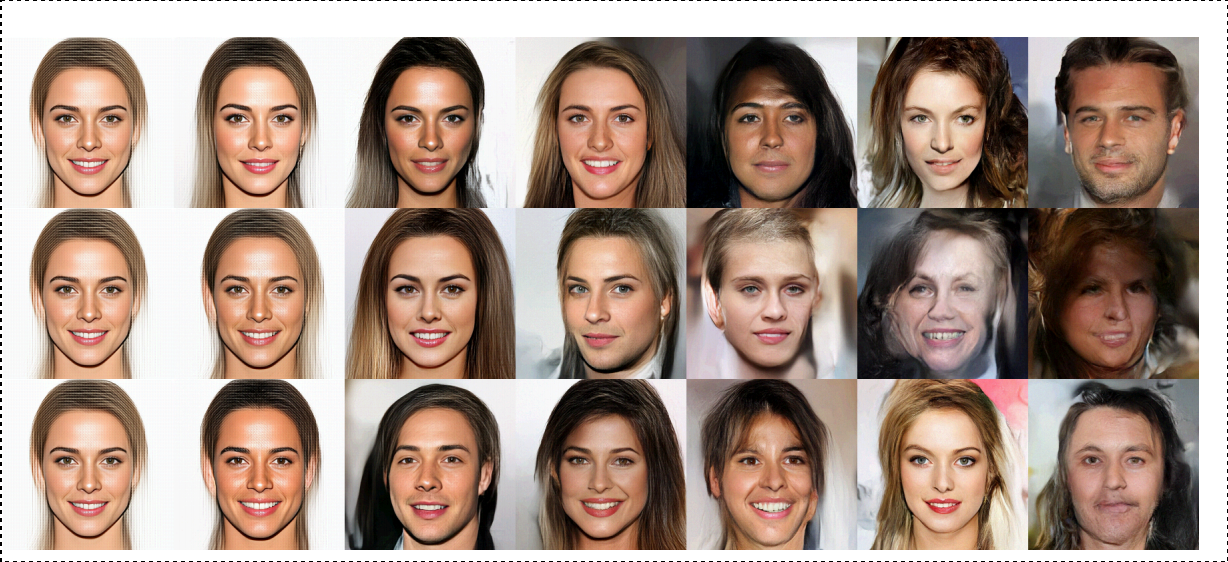
\includegraphics[width=1.0\textwidth]{glow-temperature-increase.png}
\end{frame}

\begin{frame}
  \frametitle{Effect of depth}

  Samples from shallow model on the left ($L = 4$) and deep model on the right $L = 6$.

  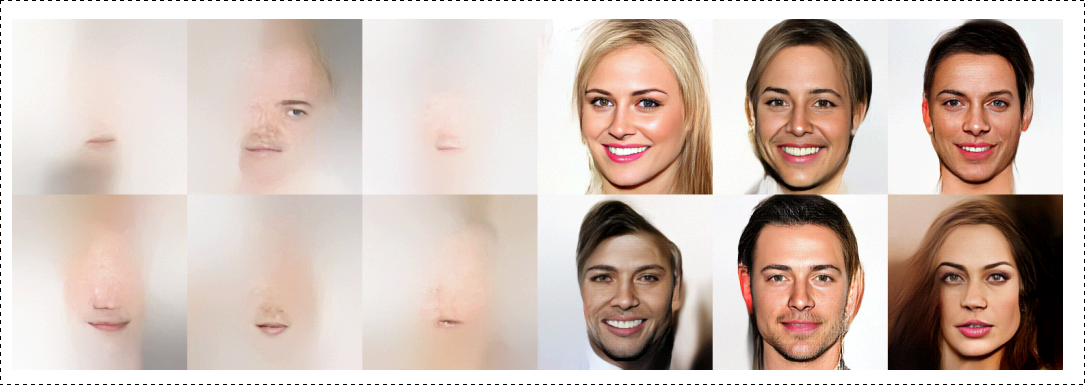
\includegraphics[width=1.0\textwidth]{glow-depth.png}
\end{frame}

\begin{frame}
  \frametitle{Progress in normalizling flows}

  Even though the model is huge and seems impractical, the progress in
  normalizing flows is quite visible.

  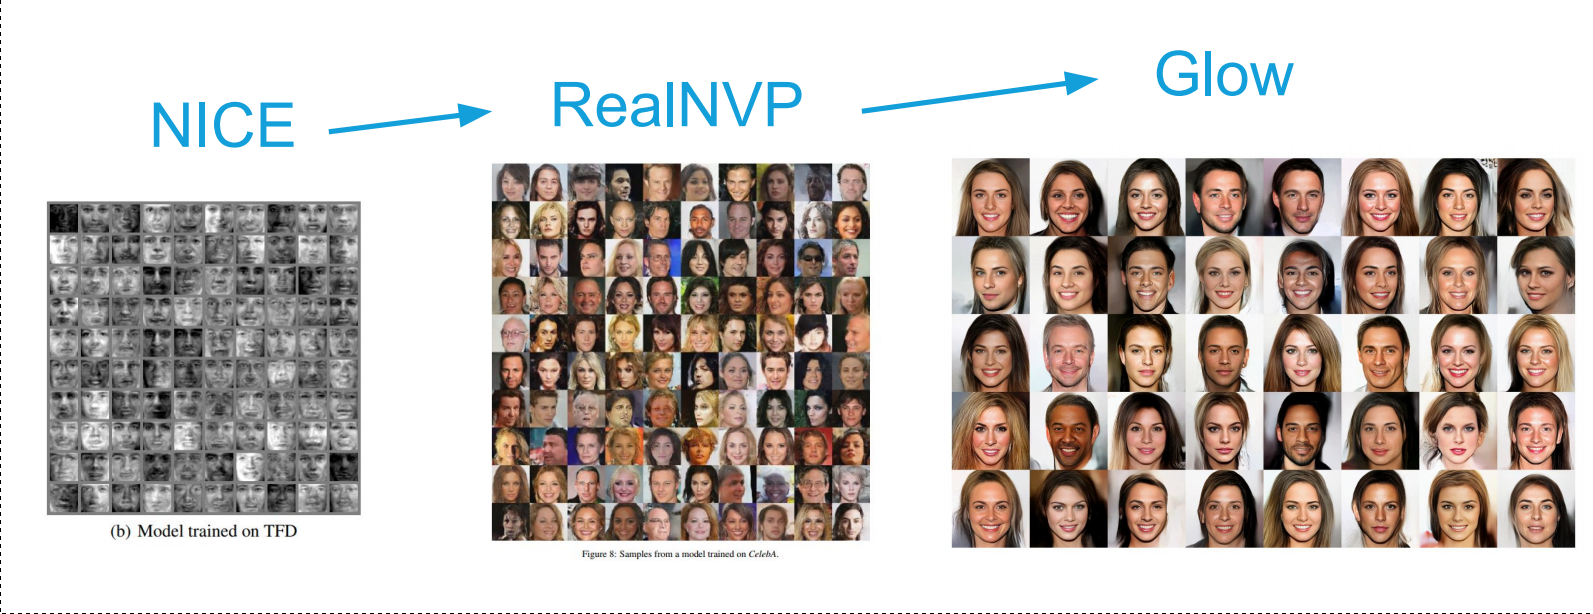
\includegraphics[width=1.0\textwidth]{normalizing-flow-progress.png}
\end{frame}


\begin{frame}
  \frametitle{Conclusion}

  \begin{aquote}{authors of the paper}
    Our model is, to the best of our knowledge, the first likelihood-based
    model in the literature that can efficiently synthesize high-resolution
    natural images.
  \end{aquote}
\end{frame}



\begin{frame}
  \frametitle{References}

  \begin{itemize}
    \item \href{https://arxiv.org/abs/1605.08803}{\beamergotobutton{Density estimation using Real NVP}}, Laurent Dinh, Jascha Sohl-Dickstein, and Samy Bengio.
    \item \href{https://arxiv.org/abs/1410.8516}{\beamergotobutton{NICE: Non-linear Independent Components Estimation}} Laurent Dinh, David Krueger, and Yoshua Bengio.
    \item \href{https://arxiv.org/abs/1807.03039}{\beamergotobutton{Glow: Generative Flow with Invertible 1x1 Convolutions}} Diederik P. Kingma, and Prafulla Dhariwal.
    \item \href{https://arxiv.org/pdf/1505.05770.pdf}{\beamergotobutton{Variational Inference with Normalizing Flows}} Danilo Jimenez Rezende, Shakir Mohamed.

    \item \href{https://lilianweng.github.io/lil-log/2018/10/13/flow-based-deep-generative-models.htm}{\beamergotobutton{Flow-based Deep Generative Models}}, Lilian Weng
    \item \href{https://blog.evjang.com/2018/01/nf1.html}{\beamergotobutton{Normalizing Flows Tutorial, Part 1: Distributions and Determinants}}, Eric Jang.
    \item \href{https://blog.evjang.com/2018/01/nf2.html}{\beamergotobutton{Normalizing Flows Tutorial, Part 2: Modern Normalizing Flows}}, Eric Jang.
    \item \href{http://akosiorek.github.io/ml/2018/04/03/norm_flows.html}{\beamergotobutton{Normalizing Flow}}, Adam Kosiorek.
    \item \href{https://github.com/kmkolasinski/deep-learning-notes/tree/master/seminars/2018-09-Introduction-to-Normalizing-Flows}{\beamergotobutton{Introduction to Normalizing Flows}}, Krzysztof Kolasinski
    \item \href{https://github.com/kmkolasinski/deep-learning-notes/tree/master/seminars/2018-10-Normalizing-Flows-NICE-RealNVP-GLOW}{\beamergotobutton{Normalizing Flows: From NICE, RealNVP to GLOW}}, Krzysztof Kolasinski
  \end{itemize}
\end{frame}

\end{document}
